\subsection{Existence and Uniqueness Theorem}
We have no guarantee that the general nonlinear system $\mathbf{\dot{x}=f(x)}$ even has solutions! This theorem helps
\begin{theorem}[\textbf{Existence and Uniqueness Theorem}]{\label{thm:eut}}
	Consider the initial value problem $\mathbf{\dot{x}=f(x)}$, $\mathbf{x}(0)=\mathbf{x}_0$. Suppose that $\mathbf{f}$ is continuous and that all its partial derivatives $\partial f_i/\partial x_j, i,j=1,\ldots,n$ are continuous for $\mathbf{x}$ in some open connected set $D\subset\mathbb{R}^n$,
	then for $\mathbf{x}_0\in D$, the initial value problem has a solution $\mathbf{x}(t)$ on some time interval $(-\tau,\tau)$ about $t=0$, and the solution is unique.
\end{theorem}
\subsection{Linear Stability Analysis in Two Dimensions}
Nodes, stars, saddles, spirals and centers are the types of fixed points that exist in linear two-dimensional dynamical systems but they also allow for a classification of the fixed points and the dynamical behavior in their neighborhoods that are found in nonlinear systems.\footnote{The important \emph{Hartmann-Grobmann theorem} states that the phase space portrait in the neighborhood of a hyperbolic fixed point is topologically equivalent to its linearization. A fixed point is called \emph{hyperbolic} if none of the real parts of its eigenvalues vanish. Such points are also called \emph{structurally stable} and a small (infinitesimal) perturbation cannot change the topology of the phase space portrait in the vicinity of a hyperbolic fixed point.}\\
To achieve classification for the nonlinear case we have to perform a linear stability analysis\footnote{Also called \emph{Linearization}.} around the fixed points in two dimensions.
\begin{equation}
	\dot{x}=f(x,y),\quad\dot{y}=g(x,y)\quad\text{with a fixed point}\quad\mathbf{\tilde{x}}=
	\begin{pmatrix}
		\tilde{x}\\\tilde{y}
	\end{pmatrix}
\end{equation}
\begin{equation*}
	\rightarrow\quad f(\tilde{x},\tilde{y})=g(\tilde{x},\tilde{y})=0
\end{equation*}
We investigate the neighborhood of the fixed point by rewriting $x$ and $y$ in the form
\begin{equation}
	\mathbf{x}=
	\begin{pmatrix}
		x\\y
	\end{pmatrix}=
	\begin{pmatrix}
		\tilde{x}+\xi\\\tilde{y}+\eta
	\end{pmatrix}\quad\rightarrow\quad
	\begin{pmatrix}
		\dot{x}\\\dot{y}
	\end{pmatrix}=
	\begin{pmatrix}
		\dot{\xi}\\\dot{\eta}
	\end{pmatrix}=
	\begin{pmatrix}
		f(\tilde{x}+\xi, \tilde{y}+\eta)\\g((\tilde{x}+\xi, \tilde{y}+\eta)
	\end{pmatrix}
\end{equation}
We now expand $f(\tilde{x}+\xi, \tilde{y}+\eta)$ and $g(\tilde{x}+\xi, \tilde{y}+\eta)$ into a Taylor series
\begin{equation}
	\begin{aligned}
		\dot{\xi}=\underbrace{f(\tilde{x},\tilde{y})}_{=0}+\ \xi\at{\frac{\partial f(x,y)}{\partial x}}{\mathbf{x=\tilde{x}}}+\eta\at{\frac{\partial f(x,y)}{\partial y}}{\mathbf{x=\tilde{x}}}+O(\xi^2,\eta^2,\xi\eta)+\cdots\\
		\dot{\eta}=\underbrace{g(\tilde{x},\tilde{y})}_{=0}+\ \xi\at{\frac{\partial g(x,y)}{\partial x}}{\mathbf{x=\tilde{x}}}+\eta\at{\frac{\partial g(x,y)}{\partial y}}{\mathbf{x=\tilde{x}}}+O(\xi^2,\eta^2,\xi\eta)+\cdots
	\end{aligned}
\end{equation}
Truncating the expansion after the linear term.
In matrix notation this linearization reads
\begin{equation}{\label{eq:j2dnls}}
	\begin{pmatrix}
		\dot{\xi}\\\dot{\eta}
	\end{pmatrix}=
	\underbrace{
	\begin{pmatrix}
		\dfrac{\partial f}{\partial x}&\dfrac{\partial f}{\partial y}\\[10pt]
		\dfrac{\partial g}{\partial x}&\dfrac{\partial g}{\partial y}
	\end{pmatrix}
	}_{\text{Jacobian}}
	\begin{pmatrix}
		\xi\\\eta
	\end{pmatrix}
\end{equation}
With Equation (\ref{eq:j2dnls}), we can treat nonlinear systems by using methods of linear systems (Section (\ref{sec:cls})).
\subsubsection{The Effect of Small Nonlinear Terms}{\label{sec:eosnt}}
As long as the fixed point for the linearized system is not one of the borderline cases discussed in Figure (\ref{fig:sumls}) we can neglect nonlinear terms.
In other words, if the linearized system predicts a saddle, node, or a spiral, then the fixed point really is a saddle, node, or spiral for the original nonlinear system.
The borderline cases (centers, degenerate nodes, stars, or non-isolated fixed
points) can be altered by small nonlinear terms.
\subsection{Potential Functions in Two-Dimensional Systems}{\label{sec:pf2d}}
A two-dimensional system of first order differential equations of the form in Equation (\ref{eq:g2de}) has a potential and is called a gradient system if there exists a scalar function of two variables $V(x,y)$ such that
\begin{equation}
	\begin{pmatrix}
		\dot{x}\\\dot{y}
	\end{pmatrix}=
	\begin{pmatrix}
		f(x,y)\\g(x,y)
	\end{pmatrix}=-
	\begin{pmatrix}
		\dfrac{\partial V(x,y)}{\partial x}\\[10pt]
		\dfrac{\partial V(x,y)}{\partial y}
	\end{pmatrix}\quad\rightarrow\quad
	\mathbf{\dot{x}}=-\nabla V(x,y)\quad\text{with}\quad\nabla=
	\begin{pmatrix}
		\dfrac{\partial}{\partial x}\\[10pt]
		\dfrac{\partial}{\partial y}
	\end{pmatrix}
\end{equation}
As in the one-dimensional case the potential function $V(x,y)$ is monotonically decreasing as time evolves.
\begin{equation}
	\dot{V}(x,y)=\underbrace{\frac{\partial V}{\partial x}}_{-\dot{x}}\underbrace{\frac{\partial x}{\partial t}}_{\dot{x}}+
	\underbrace{\frac{\partial V}{\partial y}}_{-\dot{y}}\underbrace{\frac{\partial y}{\partial t}}_{\dot{y}}=-\dot{x}^2-\dot{y}^2=-|\mathbf{\dot{x}}|^2\leq0
\end{equation}
\begin{theorem}[\textbf{Existence of a Potential in Two-Dimensional Systems}]
	A \emph{potential} exists if and only if the relation
	\begin{equation}
		\frac{\partial f(x,y)}{\partial y}=\frac{\partial g(x,y)}{\partial x}
	\end{equation}
	is fulfilled.
\end{theorem}
\subsubsection{Separatrix}
A \textbf{separatrix} is an orbit that divides the phase plane into two distinctly different types of qualitative behavior.
The homoclinic and heteroclinic orbits are examples of separatrix cycles.
\paragraph{Homoclinic Orbit}
A closed trajectory that starts and ends at the same fixed point is correspondingly called a \emph{homoclinic orbit}.\\
Consider the system
\begin{equation}{\label{eq:ho}}
	\begin{aligned}
		\dot{x}&=y-y^2\\
		\dot{y}&=x
	\end{aligned}\quad\rightarrow\quad
	\mathbf{\tilde{x}}_1=
	\begin{pmatrix}
		0\\0
	\end{pmatrix}\quad
	\mathbf{\tilde{x}}_2=
	\begin{pmatrix}
		0\\1
	\end{pmatrix}
\end{equation}
with the Jacobian Matrix
\begin{equation}
	J=\begin{pmatrix}
		0&1-2y\\1&0
	\end{pmatrix}\quad\rightarrow\quad
	J(\mathbf{\tilde{x}}_{1,2})=
	\begin{pmatrix}
		0&\pm1\\1&0
	\end{pmatrix}
\end{equation}
At $(0,0)$, $t_r[J(\mathbf{\tilde{x}})]=0$ and $d_{et}[J({\mathbf{\tilde{x}}})]=-1$ so, origin is saddle point.\\
At $(0,1)$, $t_r[J(\mathbf{\tilde{x}})]=0$ and $d_{et}[J({\mathbf{\tilde{x}}})]=1$, it is center.\\
The trajectory leaves $\mathbf{\tilde{x_1}}$ along the unstable direction, curves around the center $\mathbf{\tilde{x_2}}$ and returns along the stable direction of the saddle (Figure (\ref{fig:ho})).
\begin{figure}[h!]
	\centering
	\begin{subfigure}{0.328125\linewidth}
		\centering
		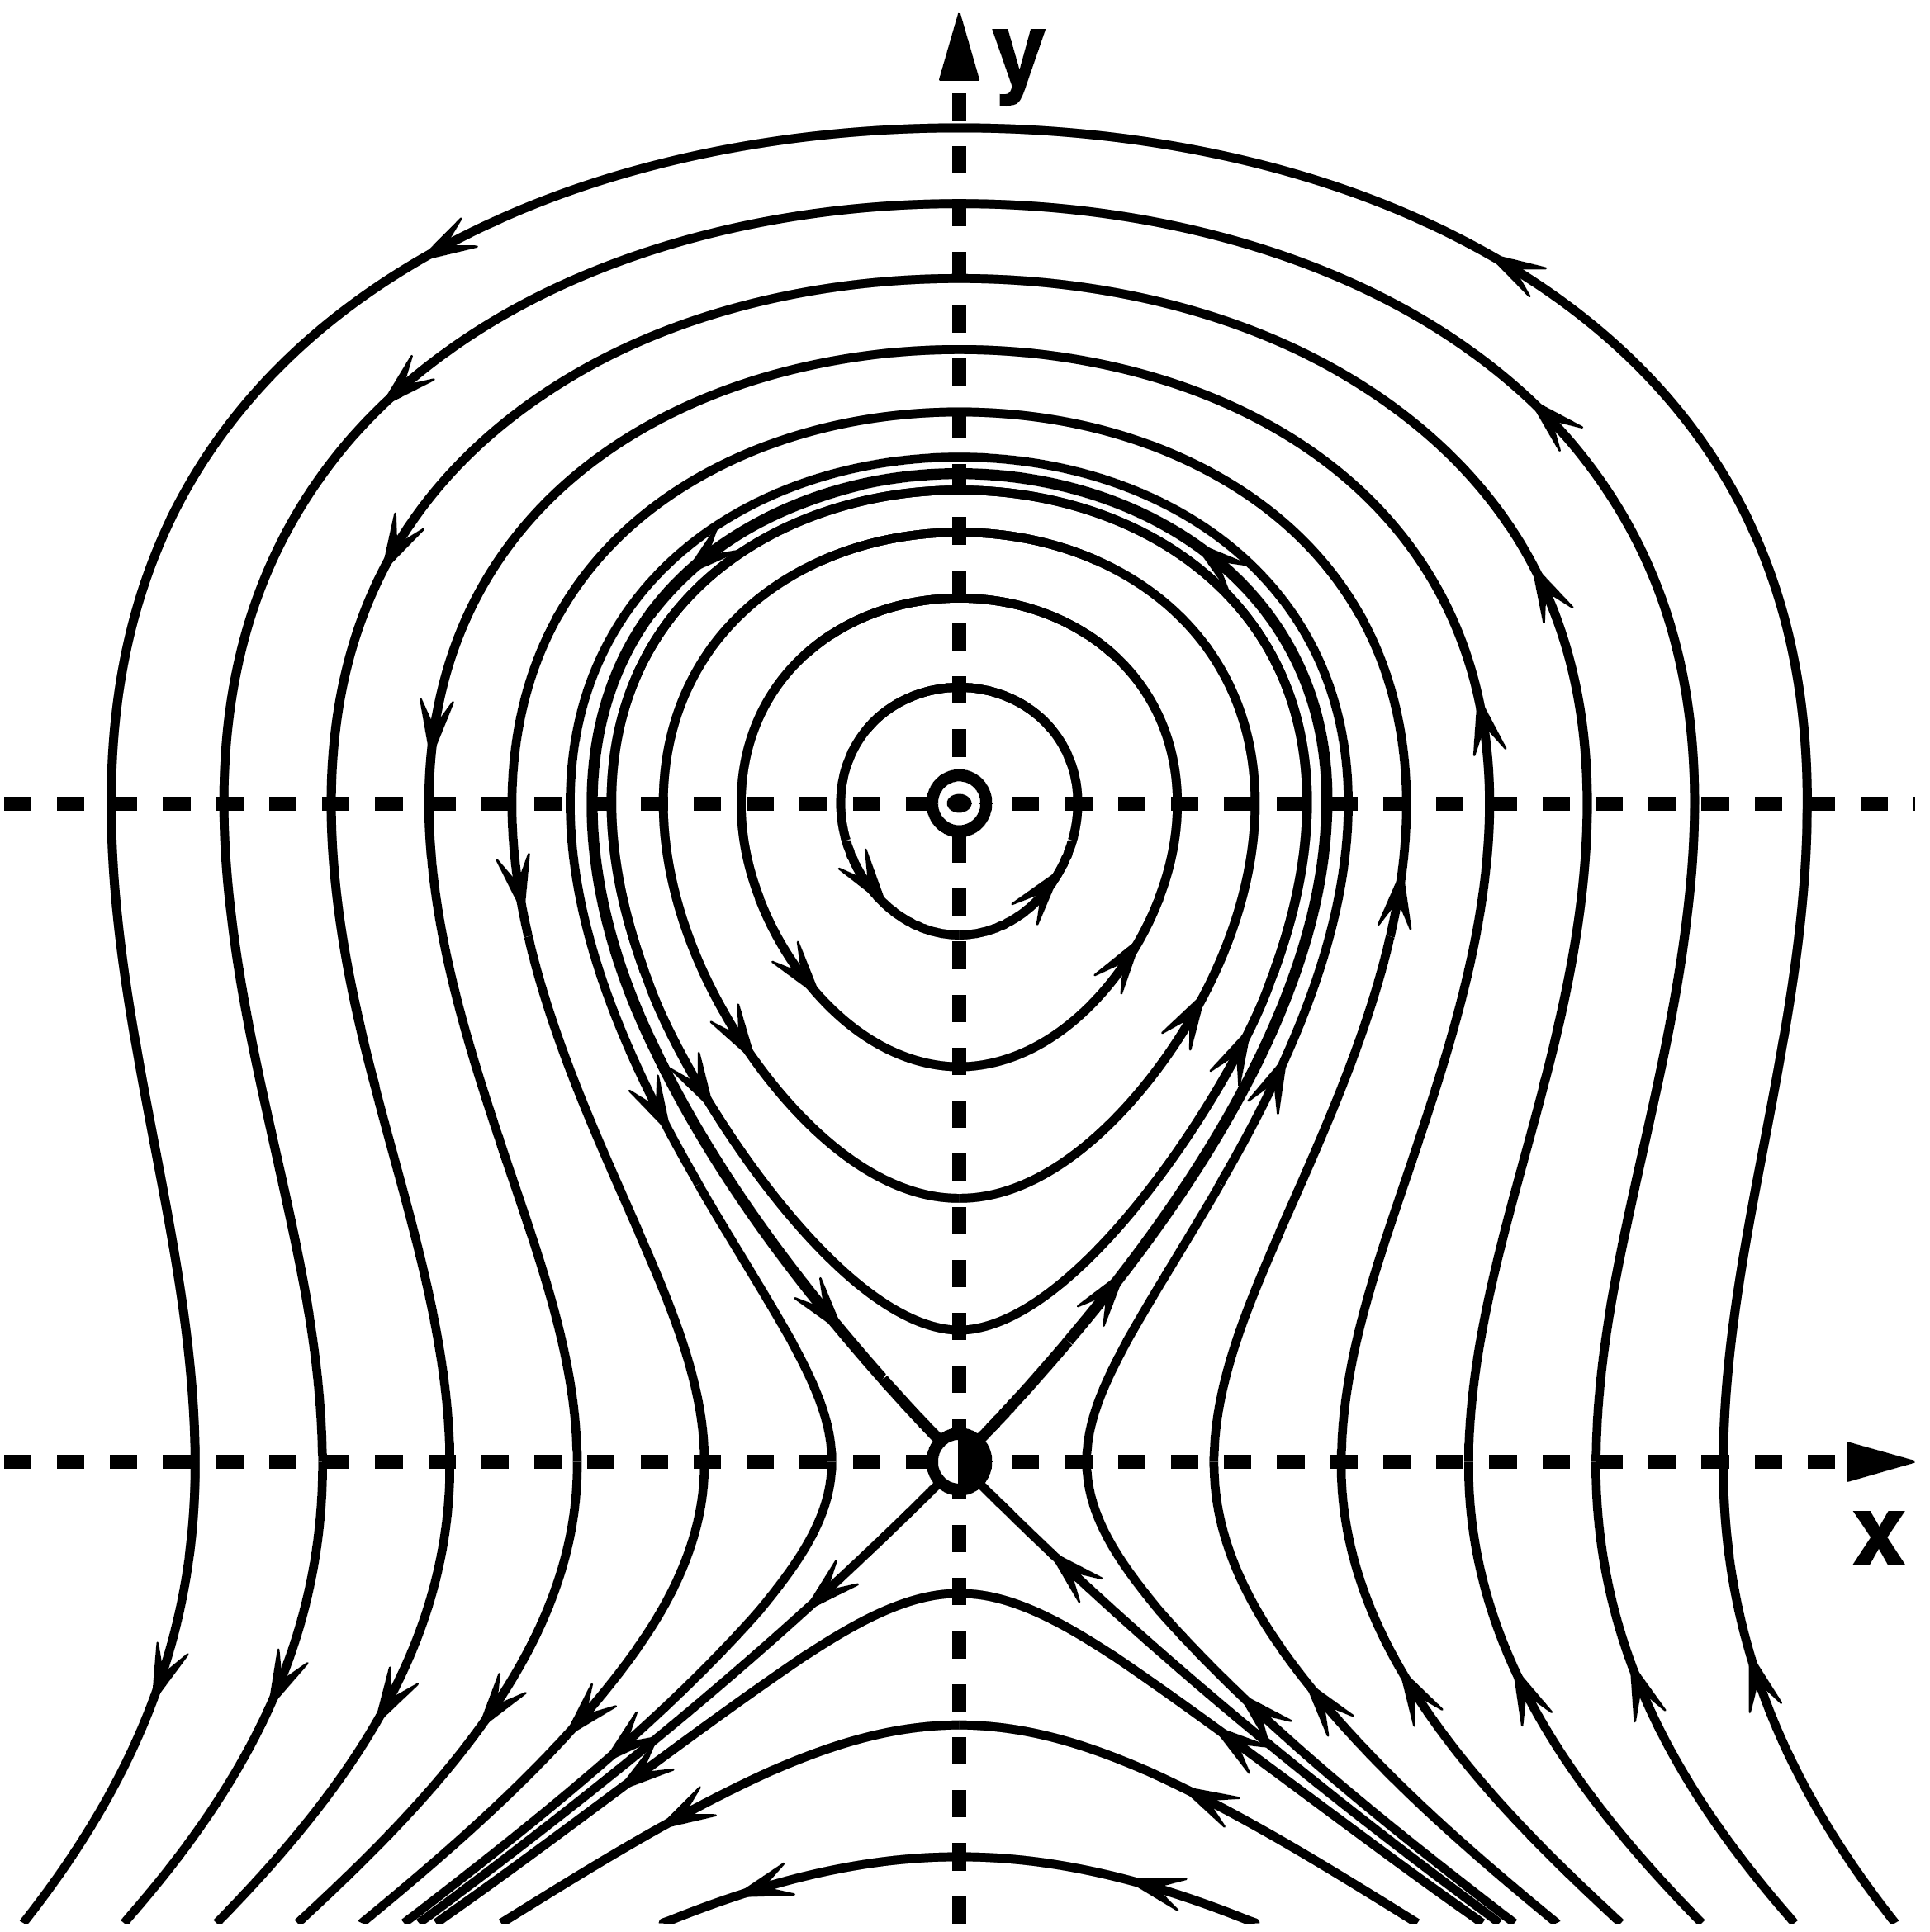
\includegraphics[width=\linewidth]{ho.png}
		\caption{Phase Space Plot of System (\ref{eq:ho})}
		\label{fig:ho}
	\end{subfigure}
	\vline
	\begin{subfigure}{0.35\linewidth}
		\centering
		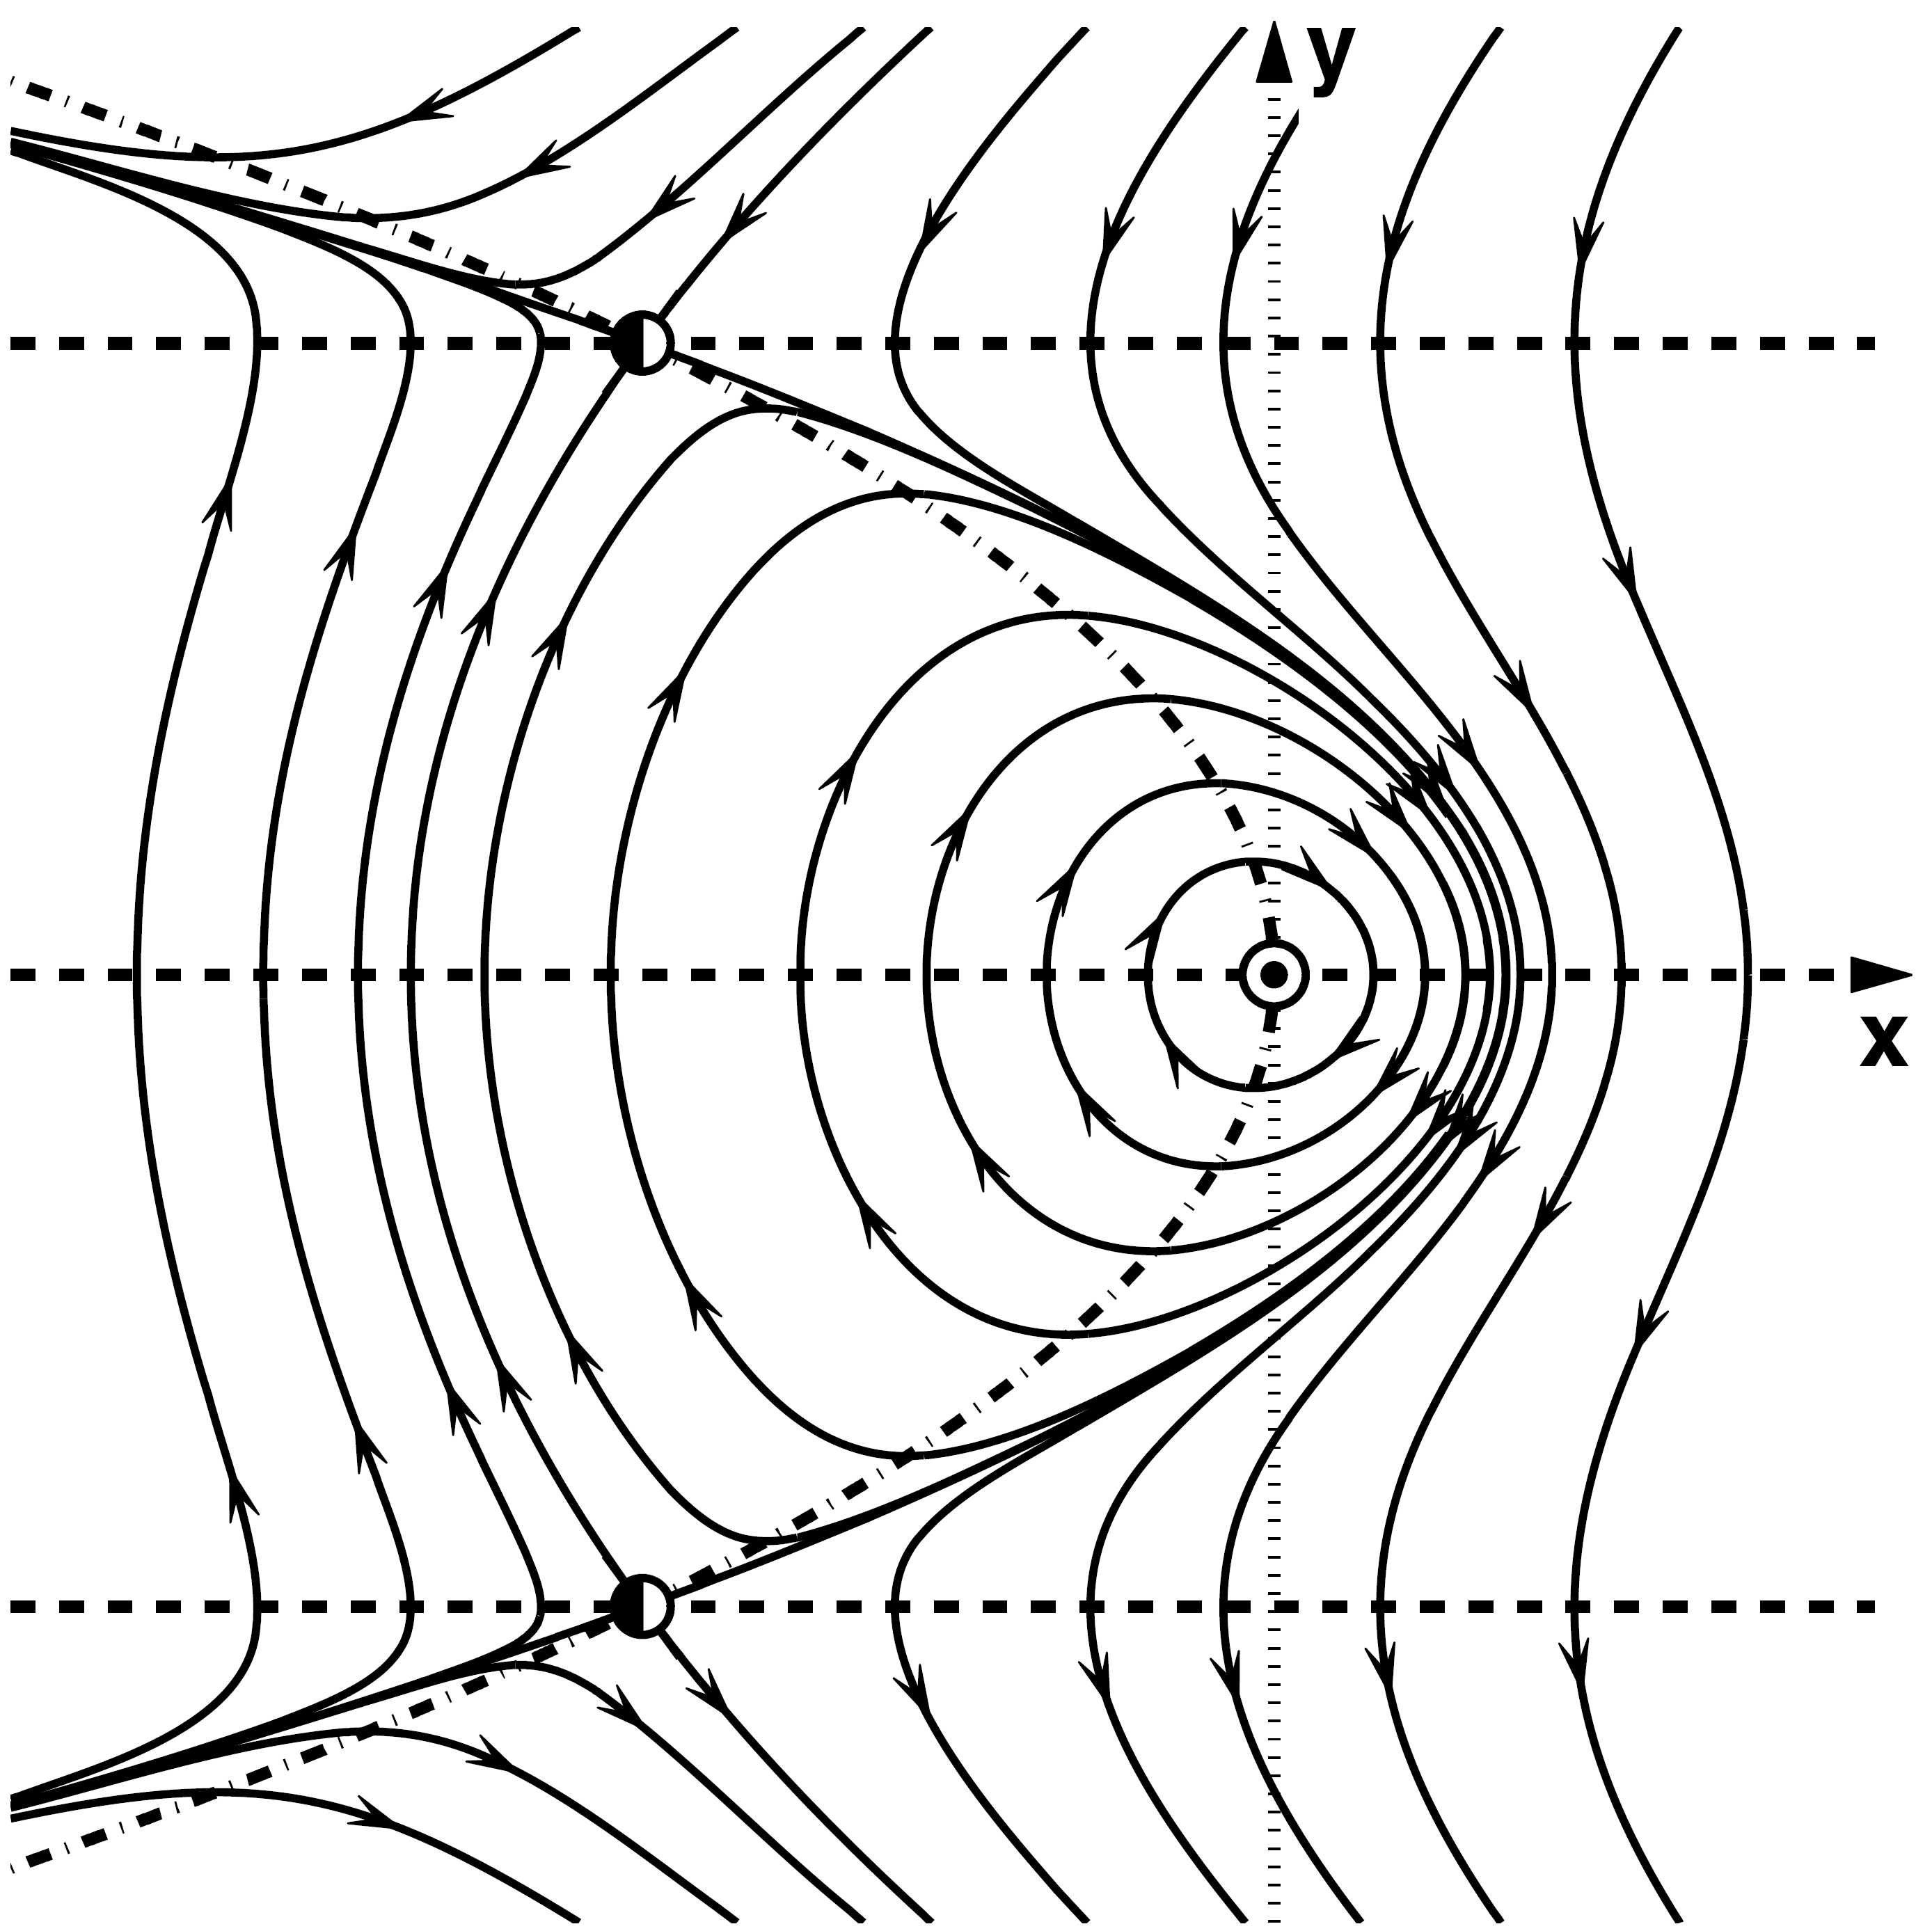
\includegraphics[width=\linewidth]{hto.png}
		\caption{Phase Space Plot of System with\\ \centering{$\dot{x}=y-y^3,\quad\dot{y}=-x-y^2$} }
		\label{fig:hto}
	\end{subfigure}
	\caption{Types of Orbits}
	\label{fig:nlo}
\end{figure}
\paragraph{Heteroclinic Orbit}
The trajectories connecting between two fixed points are called \emph{heteroclinic orbits} or \emph{saddle connections} (Figure (\ref{fig:hto})).
\subsection{Index Theory}
Linearization is a local method, it can’t tell us what happens to the trajectories after they leave that tiny neighborhood.
\emph{Index theory}, a method that provides global information about the phase portrait.
\subsubsection{The Index of a Closed Curve}
The index of a closed curve C is an integer that measures the winding of the
vector field on C.
The index also provides information about any fixed points that might happen to lie inside the curve.\\
Suppose that $\mathbf{\dot{x}=f(x)}$ is a smooth vector field on the phase plane.
Consider a closed curve $C$.
This curve is not necessarily a trajectory, it’s simply a loop that we’re putting in the phase plane to probe the behavior of the vector field.
We also assume that C is a “simple closed curve” (i.e., it doesn’t intersect itself) and that it doesn’t pass through any fixed points of the system.
Then at each point $\mathbf{x}$ on $C$, the vector field $\dot{x}=(\dot{x},\dot{y})$ makes angle $\phi=\tani(\dot{y}/\dot{x})$ with the positive $x-$axis.\\
As $\mathbf{x}$ moves counterclockwise around $C$, the angle $\phi$ changes \emph{continuously} since the vector field is smooth.
Also, when $\mathbf{x}$ returns to its starting place, $\phi$ returns to its original direction.
Hence, over one circuit, $\phi$ has changed by an integer multiple of $2\pi$. Let $[\phi]_C$ be the net change in $\phi$ over one circuit.
Then the \emph{index of the closed curve $C$ $(I_C)$} with respect to the vector field $\mathbf{f}$ is defined as
\begin{equation}
	I_C=\frac{1}{2\pi}[\phi]_C
\end{equation}
Thus, $I_C$ is the net number of counterclockwise revolutions made by the vector field as $\mathbf{x}$ moves once counterclockwise around $C$.
\subsubsection{Index of a Point}
Suppose $\mathbf{\tilde{x}}$ is an isolated fixed point.
Then the index $I$ of $\mathbf{\tilde{x}}$ is defined as $I_C$, where $C$ is any closed curve that encloses $\mathbf{\tilde{x}}$ and no other fixed points.
By property (1) below, $I_C$ is independent of $C$ and is therefore a property of $\mathbf{\tilde{x}}$ alone.
\begin{itemize}
	\item The index $I=+1$ for stable node, unstable node, spirals, centers, degenerate nodes and stars.
	\item The index $I=-1$ for saddle.
\end{itemize}
\subsubsection{Properties of the Index}
\begin{itemize}
	\item Suppose that $C$ can be continuously deformed into $C^\prime$ without passing through a fixed point.
	Then $I_C=I_{C^\prime}$
	\item If $C$ doesn’t enclose any fixed points, then $I_C=0$.
	\item If we reverse all the arrows in the vector field by changing $t\rightarrow-t$, the index is unchanged.
	Therefore, the index is not related to stability.
	\item Suppose that the closed curve $C$ is actually a trajectory for the system, i.e., $C$ is a closed orbit.
	Then $I_C=1$.
\end{itemize}
\begin{theorem}
	If a closed curve $C$ surrounds $n$ isolated fixed points $\mathbf{\tilde{x}}_1,\ldots,\mathbf{\tilde{x}}_n$ then
	\begin{equation}
		I_C=I_1+I_2+\cdots+I_n
	\end{equation}
	Where $I_k$ is the index of $\mathbf{\tilde{x}}_k$, for $k=1,\ldots,n$
\end{theorem}
\begin{theorem}
	Any closed orbit in the phase plane must enclose fixed points whose \emph{indices sum to} $+1$.
\end{theorem}